
\documentclass[border=8pt, multi, tikz]{standalone} 
\usepackage{import}
\subimport{../layers/}{init}
\usetikzlibrary{positioning}
\usetikzlibrary{3d} %for including external image 


\definecolor{ConvColor}{HTML}{4CAF50}
\definecolor{ConvReluColor}{HTML}{4CAF50}
\definecolor{PoolColor}{HTML}{B0BEC5}
\definecolor{UnpoolColor}{HTML}{B39DDB}
\definecolor{FcColor}{HTML}{1976D2}
\definecolor{FcReluColor}{HTML}{1976D2}
\definecolor{DcnvColor}{HTML}{1976D2}
\definecolor{SoftmaxColor}{HTML}{1976D2}
\definecolor{SumColor}{HTML}{FFB300}
\definecolor{PostConvColor}{HTML}{1976D2}

\def\ConvColor{ConvColor}
\def\ConvReluColor{ConvReluColor}
\def\PoolColor{PoolColor}
\def\UnpoolColor{UnpoolColor}
\def\FcColor{FcColor}
\def\FcReluColor{FcReluColor}
\def\DcnvColor{DcnvColor}
\def\SoftmaxColor{SoftmaxColor}
\def\SumColor{SumColor}
\def\PostConvColor{PostConvColor}

\def\DcnvColor{rgb:blue,5;green,2.5;white,5}
\newcommand{\copymidarrow}{\tikz \draw[-Stealth,line width=0.8mm,draw={rgb:blue,4;red,1;green,1;black,3}] (-0.3,0) -- ++(0.3,0);}

\begin{document}
\begin{tikzpicture}
\tikzstyle{connection}=[ultra thick,every node/.style={sloped,allow upside down},draw=\edgecolor,opacity=0.7]
\tikzstyle{copyconnection}=[ultra thick,every node/.style={sloped,allow upside down},draw={rgb:blue,4;red,1;green,1;black,3},opacity=0.7]
\node[canvas is zy plane at x=0] (inp) at (-3.0,0.0,0.0) {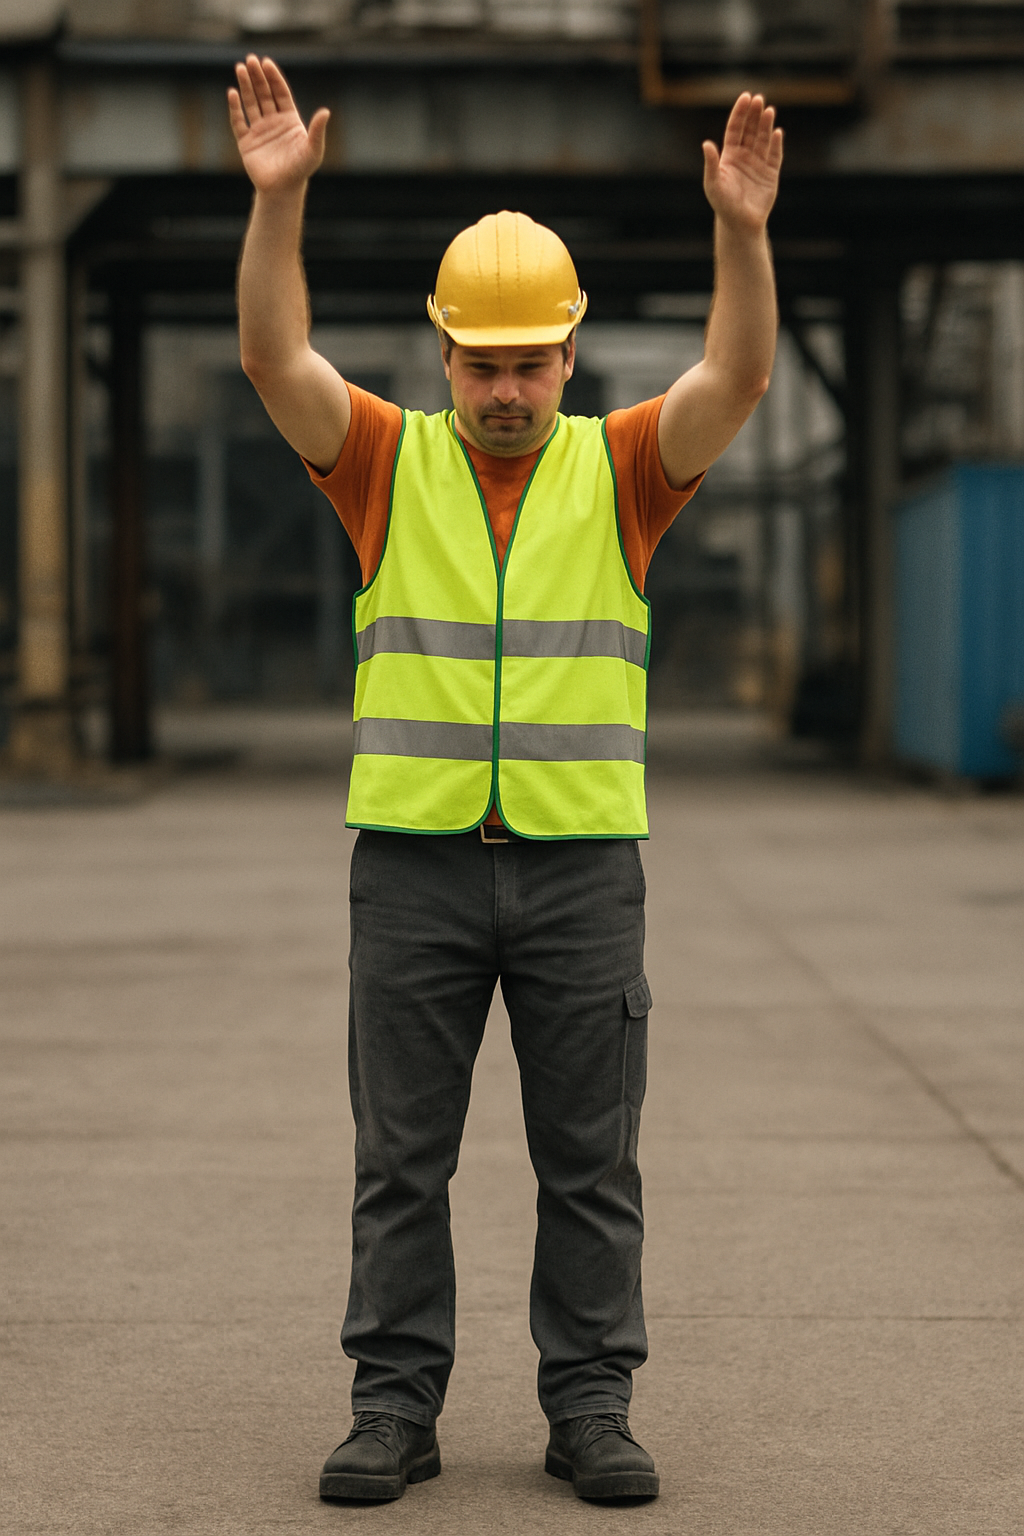
\includegraphics[width=8.0cm,height=8.0cm]{\detokenize{imgs/in.png}}};\pic[shift={(0,0,0)}] at (0,0,0) {RightBandedBox={name=cr1,caption=conv1,xlabel={{"64","64"}},zlabel=I,fill=\ConvColor,bandfill=\ConvReluColor,height=40,width={2,2},depth=40}};\pic[shift={(0,0,0)}] at (cr1-east) {Box={name=p1,fill=\PoolColor,opacity=0.5,height=35,width=1,depth=35}};\pic[shift={(2,0,0)}] at (p1-east) {RightBandedBox={name=cr2,caption=conv2,xlabel={{"64","64"}},zlabel=I/2,fill=\ConvColor,bandfill=\ConvReluColor,height=35,width={3,3},depth=35}};\pic[shift={(0,0,0)}] at (cr2-east) {Box={name=p2,fill=\PoolColor,opacity=0.5,height=30,width=1,depth=30}};\pic[shift={(2,0,0)}] at (p2-east) {RightBandedBox={name=cr3,caption=conv3,xlabel={{"256","256","256"}},zlabel=I/4,fill=\ConvColor,bandfill=\ConvReluColor,height=30,width={4,4,4},depth=30}};\pic[shift={(0,0,0)}] at (cr3-east) {Box={name=p3,fill=\PoolColor,opacity=0.5,height=23,width=1,depth=23}};\pic[shift={(1.8,0,0)}] at (p3-east) {RightBandedBox={name=cr4,caption=conv4,xlabel={{"512","512","512"}},zlabel=I/8,fill=\ConvColor,bandfill=\ConvReluColor,height=23,width={7,7,7},depth=23}};\pic[shift={(0,0,0)}] at (cr4-east) {Box={name=p4,fill=\PoolColor,opacity=0.5,height=15,width=1,depth=15}};\pic[shift={(1.5,0,0)}] at (p4-east) {RightBandedBox={name=cr5,caption=conv5,xlabel={{"512","512","512"}},zlabel=I/16,fill=\ConvColor,bandfill=\ConvReluColor,height=15,width={7,7,7},depth=15}};\pic[shift={(0,0,0)}] at (cr5-east) {Box={name=p5,fill=\PoolColor,opacity=0.5,height=10,width=1,depth=10}};\pic[shift={(1,0,0)}] at (p5-east) {RightBandedBox={name=cr6_7,caption=fc to conv,xlabel={{"4096","4096"}},fill=\ConvColor,bandfill=\ConvReluColor,height=10,width={10,10},depth=10}};\pic[shift={(1,0,0)}] at (cr6_7-east) {Box={name=c8,caption=fc8 to conv,xlabel={{"K","dummy"}},fill=\ConvColor,height=10,width=2,depth=10,zlabel=I/32}};\pic[shift={(2.5,0,0)}] at (c8-east) {Box={name=d32,caption=Deconv,xlabel={{"K","dummy"}},fill=\DcnvColor,height=40,width=2,depth=40}};\pic[shift={(1,0,0)}] at (d32-east) {Box={name=softmax,caption=softmax,xlabel={{"K","dummy"}},fill=\SoftmaxColor,height=40,width=2,depth=40,zlabel=I}};\draw [connection] (p1-east) -- node {\midarrow} (cr2-west);\draw [connection] (p2-east) -- node {\midarrow} (cr3-west);\draw [connection] (p3-east) -- node {\midarrow} (cr4-west);\draw [connection] (p4-east) -- node {\midarrow} (cr5-west);\draw [connection] (p5-east) -- node {\midarrow} (cr6_7-west);\draw [connection] (cr6_7-east) -- node {\midarrow} (c8-west);\draw [connection] (c8-east) -- node {\midarrow} (d32-west);\draw [connection] (d32-east) -- node {\midarrow} (softmax-west);\draw[densely dashed](c8-nearnortheast) -- (d32-nearnorthwest)(c8-nearsoutheast) -- (d32-nearsouthwest)(c8-farsoutheast)  -- (d32-farsouthwest)(c8-farnortheast)  -- (d32-farnorthwest);
\end{tikzpicture}
\end{document}
